\documentclass{article}
\usepackage[linesnumbered, ruled]{algorithm2e}
\usepackage{ tipa }
\usepackage{ amssymb }
% Automata package
\usepackage{tikz}
\usetikzlibrary{automata,positioning}

\setlength{\parindent}{0pt} % no indent in the beginning of a paragraph

% empty set package
\usepackage{amssymb}

\title{CSCE 423/823 - Homework 3}
\author{Tian Gao}
\begin{document}
\maketitle
	
% 1
1.\\
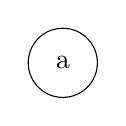
\begin{tikzpicture}[shorten >=1pt,node distance=2cm,on grid,auto] 
	\node[state] (a)   {a}; 
	;
\end{tikzpicture}\\
The statement is incorrect. \\
Consider the graph G above, V = \{a\}, E = $\varnothing$.\\
There is only one shortest path trees T = G.\\

% 2
2.\\
The statement is incorrect. \\
Consider the graph G below:\\
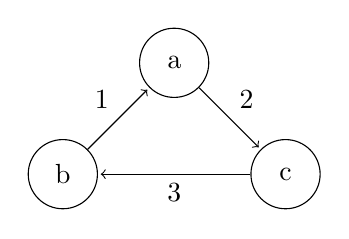
\begin{tikzpicture}[shorten >=1pt,node distance=2cm,on grid,auto] 
	\node[state] (b)   {b}; 
	\node[state] (a) [above right=of b] {a}; 
	\node[state] (c) [below right=of a] {c}; 
	\path[->] 
	(b) edge  node {1} (a)
	(a) edge  node {2} (c)
	(c) edge  node {3} (b)
	;
\end{tikzpicture}\\
So T is the following tree rooted as a:\\
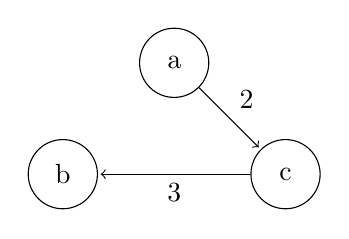
\begin{tikzpicture}[shorten >=1pt,node distance=2cm,on grid,auto] 
	\node[state] (b)   {b}; 
	\node[state] (a) [above right=of b] {a}; 
	\node[state] (c) [below right=of a] {c}; 
	\path[->] 
	(a) edge  node {2} (c)
	(c) edge  node {3} (b)
	;
\end{tikzpicture}\\
So G' is the following graph:\\
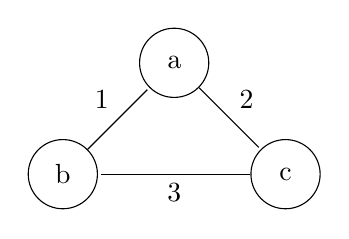
\begin{tikzpicture}[shorten >=1pt,node distance=2cm,on grid,auto] 
	\node[state] (b)   {b}; 
	\node[state] (a) [above right=of b] {a}; 
	\node[state] (c) [below right=of a] {c}; 
	\path[-] 
	(b) edge  node {1} (a)
	(a) edge  node {2} (c)
	(c) edge  node {3} (b)
	;
\end{tikzpicture}\\
T' is the following tree:\\
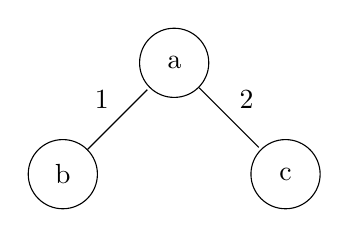
\begin{tikzpicture}[shorten >=1pt,node distance=2cm,on grid,auto] 
	\node[state] (b)   {b}; 
	\node[state] (a) [above right=of b] {a}; 
	\node[state] (c) [below right=of a] {c}; 
	\path[-] 
	(b) edge  node {1} (a)
	(a) edge  node {2} (c)
	;
\end{tikzpicture}\\
Obviously, T $\neq$ T'.

% 3
3. \\
The statement can be proved by contradiction.\\
Suppose $T''$ rather than $T'$ is the MST of $G'$ and $T'' \neq T'$.\\
Assume $E'$ includes all the edges in T and not in $T'$.\\
Then $T''' = E' \cup T''$ is a MST of G since T is the MST of G and $T'$ is connected.\\
Since $T''$ is a MST of $G'$, $w(T'') < w(T')$.\\
So $w(T''') = w(E' \cup T'') = w(E') + w(T'') < w(E') + w(T') = w(E' + T') = w(T)$\\
So T is not a MST since there is another spanning tree having lighter weight.\\
Contradiction!\\

% 4
4.\\
Since the weight of an edge is at most W, a shortest-path estimate is at most $(|V| - 1)W$ if it is not $\infty$.\\
So we can use a prioritization queue to store all the vertices based on the estimated distance.\\
The queue includes $(|V| - 1)W$ buckets and vertex v is in bucket v.d.\\
The starting vertex s is in bucket 0, and all the vertices with distance $\infty$(undiscovered vertices) are in the last bucket.\\
After initialization, we can go through all the buckets from 0 to $(|V| - 1)W$.\\
If the current bucket is empty, we skip it. Otherwise, we go through all the vertices in that bucket and relax their adjacent vertices.\\
This process is repeated until the last bucket is reached. After that, we have all the vertices with shortest path in the buckets.\\
As for the time complexity, scanning the prioritization queue cost $O(W|V|)$. Going through all the vertices in each buckets totally cost $O(|V|)$.
Relaxing the adjacent vertices totally cost $O(|E|)$.\\
So the total time complexity is $O(W|V| + |V| + |E|)=O(W|V| + |E|)$\\

% 5
5.\\
\begin{algorithm}[H]
	\caption{BELLMAN-FORD-MOD(G, w, s)}
	INITIALIZE-SINGLE-SOURCE(G, s)\;
	flag = TRUE\;
	\While{flag == TRUE}
	{
		flag = FALSE\;
		\For{each edge (u, v) $\in$ G.E}
		{
			RELAX-MOD(u, v, w)
		}
	}
\end{algorithm}

\begin{algorithm}[H]
	\caption{RELAX-MOD(u, v, w)}
	\If{v.d $>$ u.d + w(u, v)}
	{
		v.d = u.d + w(u, v)\;
		v.$\pi$ = u\;
		flag = TRUE\;
	}
\end{algorithm}
Explanation:\\
According to Lemma 24.2(ref[1]), since m is the maximum number of edges in a shortest path, all the vertices reachable from source s 
achieved the shortest-path distance v.d after m iterations.\\
So, in the m+1 iteration, v.d will not change any more.\\
So we can use a flag to detect whether v.d is changed. If there is no change, we must be in the m+1 iteration.\\

Ref:\\
1. Page 652, Introduction to Algorithms, Third Edition by Thomas H. Cormen, Charles E. Leiserson, Ronald L. Rivest, and Clifford Stein, MIT Press, 2009.\\
2. Chen, J. (2018). CLRS Solutions. [online] Walkccc.github.io. Available at: https://walkccc.github.io/CLRS [Accessed 30 Jul. 2018].

% 6
6.\\
We can modify the Ford-Fulkerson algorithm to get the maximum benefit path.\\
\begin{algorithm}[H]
	\caption{FORD-FULKERSON-MOD(G, s, t)}
	\For{each edge(u, v) $\in$ G.E}
	{
		(u, v).f = 0
	}
	\While{there exists a path p from s to t in the residual network $G_f$}
	{
		$c_f(p)$=min{w(u, v) - benefit(u, v): (u, v) is in p}\;
		\For{each edge (u, v) in p}
		{
			(u, v).f = min((u, v).f, $c_f(p)$)
		}
	}
\end{algorithm}
Explanation:\\
Similar to Ford-Fulkerson algorithm, the algorithm above is looking for the better paths that have a better benefit. \\
The only difference is the way to update flow. 

Time complexity:\\
Similar to Ford-Fulkerson algorithm, the time complexity is $O(E|f^*|)$.\\


\end{document}
